\begin{figure}[!htp]
    \centering
    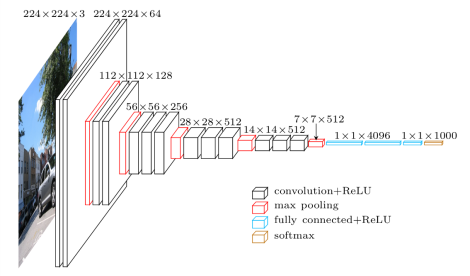
\includegraphics[width=\textwidth]{Images/vgg16.png}
    \caption{VGG16 Model Architecture}
\end{figure}

The VGG16 model is heavy model architecture containing 16 layers in the 
model. The model architecture consist of 13 convolutional, 5 pooling and 3 fully connected 
layers. Due to the heavy model architecture with estimated 138 million parameters
and limited hardware resources it was not possible to trian the model on personal machine. As, a result the google colab platform was used develop
the convolutional network \footnote{\url{https://colab.research.google.com/drive/1QHIHhu28sSiW0T-ZGTwg0bp-bulW30l1}}.

\begin{figure}[!htp]
    \centering
    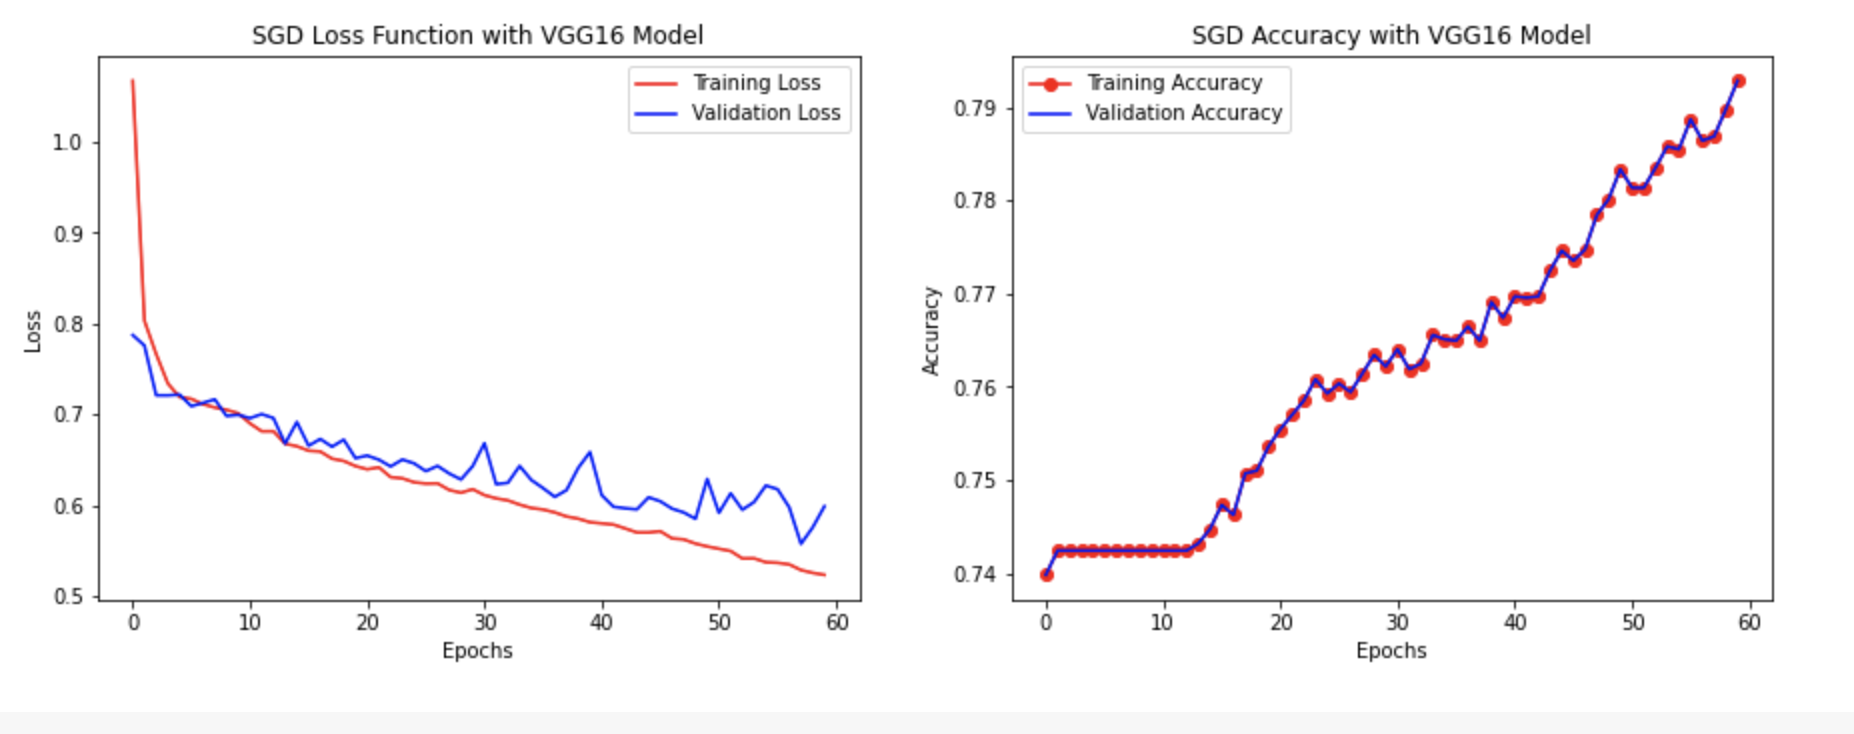
\includegraphics[width=\textwidth]{Images/vgg16Results.png}
    \caption{VGG16 Model Architecture}
    \label{fig:vggRes}
\end{figure}
The figure \ref{fig:vggRes} shows the graph of model accuracy increasing over the 
epochs and decline in the loss function. The VGG model was trained using the SGD optimiser and learning 
rate of 0.01 which resulted in accuracy of 78.14\% over the 60 epochs. 
\subsection{Transfer Learning with VGG16}
Another, test was performed to evaluate the performance of the model with transfering the
weights obtained from the model mentioned above for 300 epochs.

\begin{figure}[!htp]
    \centering
    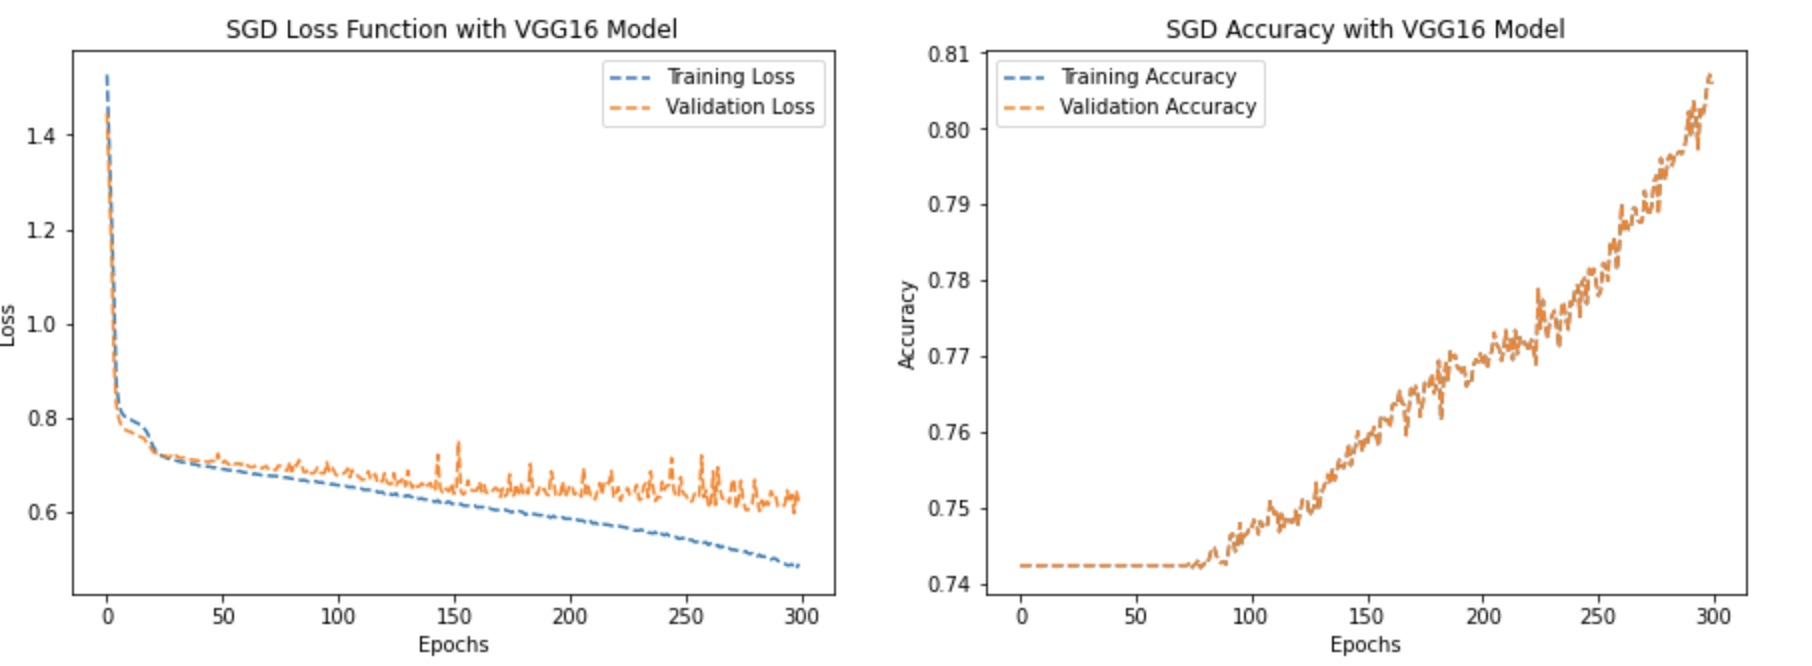
\includegraphics[width=\textwidth]{Images/vgg162.png}
    \caption{VGG16 Model Architecture}
    \label{fig:vggRes2}
\end{figure}

In the figure \ref{fig:vggRes2} the training and validation accuracy 
was increasing with same growth with increase in the number of epochs.
The result obtained from the experiment was 77.48\% on testing data which is 
worst then the evaluation of the previous model. The poor model accuracy could be a result 
of overfitting of the convolutional network.
